
\makeatletter
\begin{titlepage}

\thispagestyle{empty}

\includegraphics[width=0.6\textwidth]{images/zhaw_lsfm_iunr_schwarz.jpg}

\begin{center}

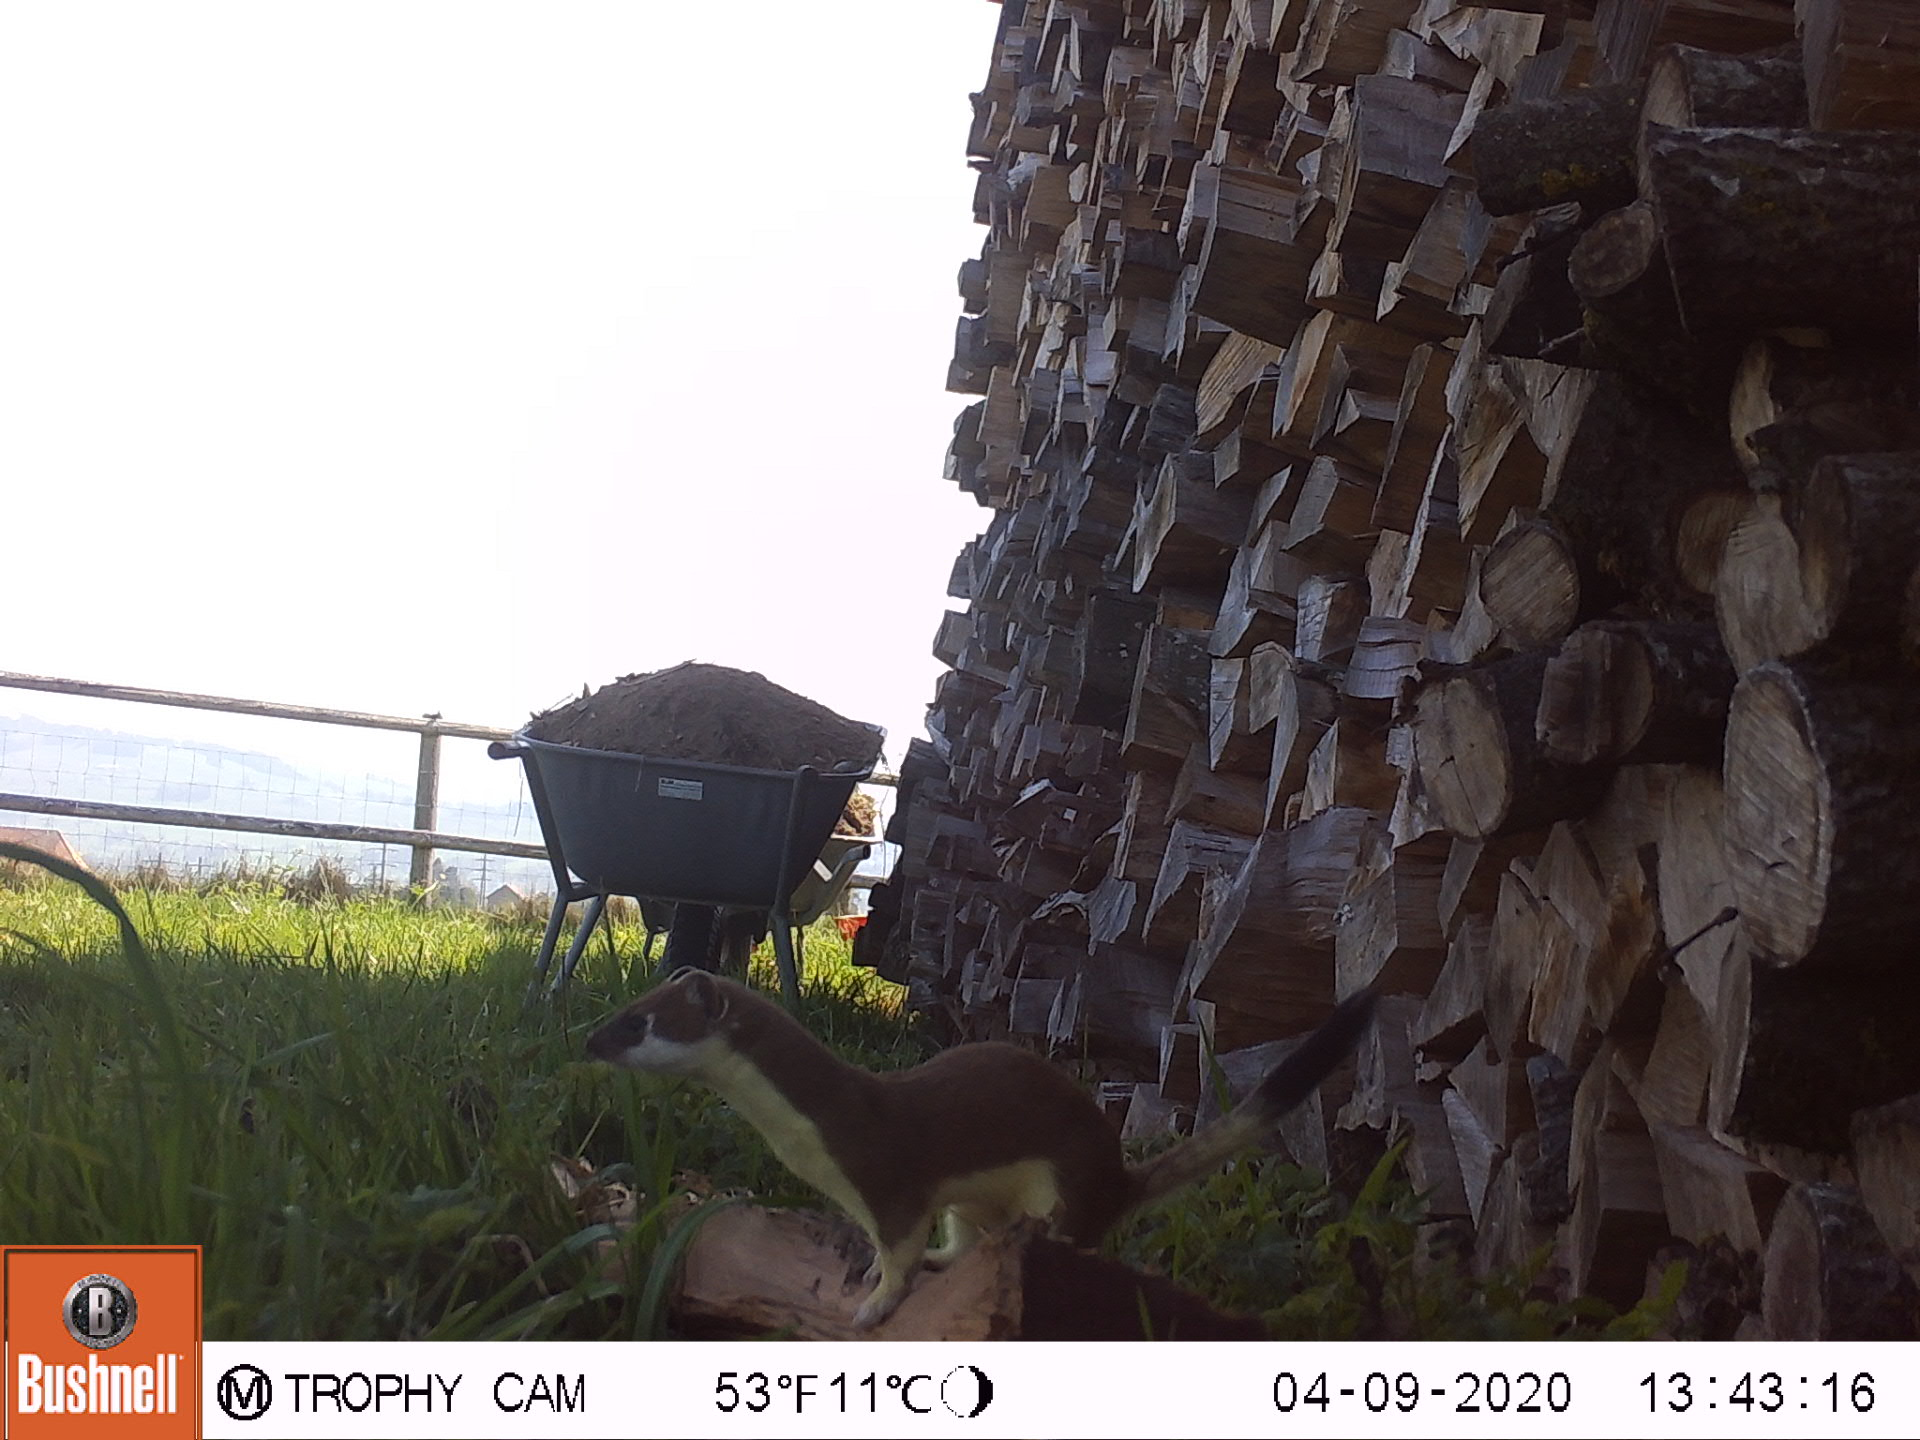
\includegraphics{images/Hermelin_Str116_WK02.JPG}

\vspace{10pt}

{\huge \@title}

\vspace{30pt}

% {\Large \@subtitle}
% 
% {\Large \@date}



\end{center}



\begin{flushleft}

% \begin{table}[]
\begin{minipage}{21cm}
\vspace{10cm}


\begin{tabular}{ll}
Auftraggeber: & \textbf{Wiesel \& Co am Zimmerberg}                         \\
              & c / o Stefan Keller                                         \\
              & Aeschstrasse 23,                                            \\
              & 9122 Mogelsberg                                             \\
              &                                                             \\
Bearbeitung:  & \textbf{Institut für Umwelt und Natürliche Ressourcen IUNR} \\
              & ZHAW Zürcher Hochschule für Angewandte Wissenschaften       \\
              & Life Sciences und Facility Management                       \\
              & Forschungsgruppe Geoinformatik                              \\
              & Grüental, Postfach                                          \\
              & CH-8820 Wädenswil                                           \\
              &                                                             \\
Autoren:      & Nils Ratnaweera\textsuperscript{1}                         \\
              & Inga Laas\textsuperscript{2}                              \\
              & Silvio Aegerter\textsuperscript{2}                        \\
              & Patrick Laube\textsuperscript{1}                           \\
              &                                                             \\
              & \textsuperscript{1} ZHAW, \textsuperscript{2} Wiesel \& Co am Zimmerberg \\
              &                                                             \\
              &                                                             \\
Titelbild:    & Hermelin vor einem Winterquartier (Laas, 2020)                
\end{tabular}
% \end{table}
\end{minipage}


\end{flushleft}

\end{titlepage}
\makeatother


\let\maketitle\oldmaketitle


